\chapter{Diferenciación Automática}\label{chapter: AD}

Para obtener la estructura automática que evalúe cada variante de VRP, así como los problemas vecinos, que se obtienen cuando se aplican los criterios de vecindad, sin necesidad de reestructurar el código, se utiliza una cinta computacional. Esta cinta se aplica, de manera similar, en el proceso matemático de Diferenciación Automática (AD, por sus siglas en inglés) y se explica en este capítulo.

Este capítulo está dividido en 5 secciones. La sección \ref{2:AD-process} trata sobre el concepto de diferenciación automática. La sección \ref{2:eval-modes} presenta y describe los dos modos de evaluación de esta estrategia. La sección \ref{2:tape} presenta la estructura de la cinta de evaluación que utiliza AD.
\section{Proceso de Diferenciación Automática (AD)}\label{2:AD-process}
En esta sección se presenta el concepto y las caraterísticas de la Diferenciación Automática.

AD es una estrategia que se utiliza para evaluar la derivada de una función matemática a través de un código computacional. Se utiliza la regla de la cadena y se obtiene la evaluación de las derivadas sin errores numéricos.

La información durante el proceso de evaluación se guarda en variables intermedias, dentro de una cinta de evaluación, que no es más que el registro de una corrida en particular de un programa dado, con valores particulares especificados para las variables de entrada, mostrando la secuencia de valores intermedios calculados y las operaciones realizadas. A esta cinta de evaluación también se le conoce con el nombre de \textbf{procedimiento de evaluación}. En caso de una reestructuración de la función inicial, se mantendrá guardada la información de las partes no alteradas de la función. Estas partes no modificadas de la función no se vuelven a evaluar y de esta manera no se repiten cálculos innecesarios. A continuación se muestra un ejemplo de cómo se usa esta estrategia de evaluación:

Sea la función $y = f(x1,x2)$ donde:
\begin{equation}
	\label{eq:example}
y = tan(x1) * \frac{x1}{x2} + sen(x2) * cos(x1)
\end{equation}

Se quiere calcular el valor de $y$ en algún punto $(x_{1}^{*},x_{2}^{*})$.
El Cuadro \ref{tab:table1} muestra la manera en la que se evalúa la función aplicando esta estrategia de evaluación automática. Se muestra una secuencia de variables, las primeras son variables de entrada; luego siguen las intermedias (denotadas por $V_{i}$ con $i>0$),y al final las de salida (en este caso es $y$). Cada variable es calculada a partir de aquellas definidas previamente aplicando una de las operaciones o funciones elementales: suma, resta, multiplicación, seno, exp, etc.

El procedimiento de evaluación no se corresponde directamente con la expresión de $f$ como fue escrita originalmente, sino con una expresión cuya evaluación es más eficiente mediante sub-expresiones repetidas, evaluadas una vez, y luego reutilizadas. El procedimiento de evaluación captura la secuencia precisa de operaciones y argumentos usados por una implementación particular de un algoritmo o función. Las expresiones generadas serán reutilizadas para la evaluación de las derivadas.

\begin{table}[h]
\begin{center}
\begin{tabular}{|l|} \hline
			$\begin{aligned}
			v_{-1} & = x_{1}	   \\
			v_{0}  & = x_{2}\\
			\end{aligned}$   	
			\\ \hline
			
			$\begin{aligned}
			\ \ v_{1} & = tan(v_{-1})   \\
			\ \ v_{2} & = v_{-1}/v_{0}  \\
			\ \ v_{3} & = v_{1}*v_{2}   \\
			\ \ v_{4} & = sen(v_{0})   \\
			\ \ v_{5} & = cos(v_{-1}) \\
			\ \ v_{6} & = v_{4}*v_{5} \\
			\ \ v_{7} & = v_{3}+v_{6}\\
			\end{aligned}$
			\\ \hline
			$\begin{aligned}
			\ \ \ y &= v_{7} 
			\end{aligned}$
			\\ \hline
\end{tabular}
		\caption{Cinta para la evaluación de la función del ejemplo \ref{eq:example}}
		\label{tab:table1}
\end{center}
\end{table}

Este procedimiento utiliza un grafo computacional que se presenta en la siguiente sección.

\section{Grafo computacional}\label{2:graph}
La relación entre las variables, es decir, las dependientes e independientes se presentan en un grafo computacional, parecido al utilizado en el sistema de VRP. Para el ejemplo mostrado en esta sección aquí se tiene la Figura \ref{fig:ADgraph}.

\begin{figure}[htb]
	\centering
	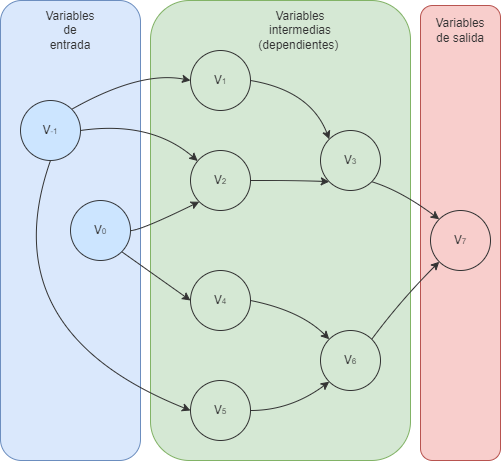
\includegraphics[width=0.5\linewidth]{Graphics/ADgraph}
	\caption{Grafo de evaluación para el ejemplo, se distinguen los diferentes tipos de variables.}.\label{fig:ADgraph}
\end{figure}
		
Como se puede notar las raíces del grafo son las variables independientes mientras que los demás nodos son variables dependientes. La diferenciación automática utiliza dos maneras básicas de propagar las derivadas a través de la cinta y así llevar la información precalculada a los siguientes niveles para su uso. Uno es el modo \textit{forward} y el otro el modo \textit{reverse} que serán tratados en la siguinte sección.

\section{Modos de evaluación}\label{2:eval-modes}

El modo forward o hacia adelante consiste en propagar derivadas desde variables independientes o de entrada, y a través de variables intermedias hasta variables dependientes o de salida del programa, siguiendo el flujo de ejecución del mismo.

De forma general, se aplica la regla de la cadena para cada variable intermedia $v_{i}$ que se calcula, almacenando los valores obtenidos en nuevas variables $v^{*}_{i}$, que a la vez se utilizan en las subsiguientes aplicaciones de la regla de la cadena a lo largo de la ejecución del programa, hasta propagar las derivadas a las variables dependientes.

Para mostrar cómo funciona el modo forward se toma el ejemplo \ref{eq:example}. El resultado se muestra en el cuadro \ref{tab:table2}.

Cada $v_{i}$ representa las variables vistas en el Cuadro \ref{tab:table1} y cada $v_{i}^{*}$ representa su derivada que será propagada.

\begin{table}[htp]
		\begin{center}
			\begin{tabular}{|l|} \hline
			$\begin{aligned}
			
			v_{-1}&=x_{1}     \\
			v_{-1}^{*}&=x_{1}^{*}	   \\
			v_{0}&=x_{2} 	   \\ 
			v_{0}^{*}&=x_{2}^{*}
			\end{aligned}$
			\\ \hline
			$\begin{aligned}
			\ \ v_{1}&=tan(v_{-1})   \\
			v_{1}^{*}&=1/cos^{2}(v_{-1})*v_{-1}^{*} \\
			v_{2}&=v_{-1}/v_{0}  \\
			v_{2}^{*}&=(v_{-1}^{*}*v_{0}-v_{0}^{*}*v_{-1})/v_{0}^{2} \\
			v_{3}&=v_{1}*v_{2}   \\
			v_{3}^{*}&=v_{1}^{*}*v_{2}+v_{2}^{*}*v_{1} \\
			v_{4}&=sen(v_{0})   \\
			v_{4}^{*}&=cos(v_{0})*v_{0}^{*}   \\
			v_{5}&=cos(v_{-1}) \\
			v_{5}^{*}&=-sen(v_{-1})*v_{-1}^{*} \\
			v_{6}&=v_{4}*v_{5} \\
			v_{6}^{*}&=v_{4}^{*}*v_{5}+v_{5}^{*}*v_{4} \\
			v_{7}&=v_{3}+v_{6} \\
			v_{7}^{*}&=v_{3}^{*}+v_{6}^{*} \\
			\end{aligned}$	
			\\ \hline
			$\begin{aligned}
			\ \ y = v_{7} \\
			\ \ y^{*} = v_{7}^{*} \\
			\end{aligned}$		
			\\ \hline
			\end{tabular}
		\caption {Procedimiento de evaluación de la derivada con el modo forward.} 
		\label{tab:table2}
		\end{center}
\end{table}

De la tabla \ref{tab:table1} a la \ref{tab:table2} se realiza un procedimiento completamente mecánico. Cada expresión original es sucedida por una correspondiente expresión derivada, de manera que la longitud del procedimiento de evaluación derivado es el doble del original.

El modo reverse o hacia atrás, una vez ejecutado el procedimiento de evaluación de la función hacia adelante, la información de las derivadas se propaga en sentido contrario al flujo de ejecución del programa, desde las variables dependientes o de salida, y a través de las variables intermedias hasta las variables independientes o de entrada.

De forma general, por cada variable intermedia $v_{i}$ se genera una variable llamada \textit{variable adjunta} $v^{*}_{i}$, que acumula incrementalmente los valores $v^{*}_{i}* \frac{\partial{y_{j}}}{\partial{v_{i}}}$ para todas las variables $v_{j}$ que dependen de $v_{i}$ donde $y_{j}$ es una función que describe precisamente esa dependencia.

A continuación se muestra el resultado de aplicar el modo reverse al ejemplo \ref{eq:example}. La fase hacia adelante es la misma que en el Cuadro \ref{tab:table1}. El resultado de la fase hacia atrás se muestra en el cuadro \ref{tab:table3}.

\begin{table}[htp]
	\begin{center}
		\begin{tabular}{|l|} \hline
			$\begin{aligned}
			v_{-1} & = x_{1}	   \\
			v_{0}  & = x_{2}\\
			\end{aligned}$   	
			\\ \hline
			
			$\begin{aligned}
			\ \ v_{1} & = tan(v_{-1})   \\
			\ \ v_{2} & = v_{-1}/v_{0}  \\
			\ \ v_{3} & = v_{1}*v_{2}   \\
			\ \ v_{4} & = sen(v_{0})   \\
			\ \ v_{5} & = cos(v_{-1}) \\
			\ \ v_{6} & = v_{4}*v_{5} \\
			\ \ v_{7} & = v_{3}+v_{6}\\
			\end{aligned}$
			\\ \hline
			$\begin{aligned}
			\ \ \ y &= v_{7} 
			\end{aligned}$
			\\ \hline
        \end{tabular}
		\begin{tabular}{|l|} \hline
		$\begin{aligned}
		\ \ v_{7}^{*} \ \ \ \ &= y^{*}
	    \end{aligned}$
	    \\ \hline
		$\begin{aligned}
		v_{6}^{*}& += v_{7}^{*}	   \\
		v_{3}^{*}& += v_{7}^{*}	   \\
		v_{5}^{*}&+= v_{4}*v_{6}^{*} \\
		v_{4}^{*}&+= v_{5}*v_{6}^{*} \\ 
		v_{-1}^{*}&+= -v_{5}^{*}*sen(v_{-1})\\
		v_{0}^{*}&+= v_{4}^{*}*cos(v_{0})\\
		v_{2}^{*}&+=v_{3}^{*}*v_{1}\\
		v_{1}^{*}&+=v_{3}^{*}*v_{2}\\
		v_{0}^{*}&+= \frac{-v_{2}^{*}*v_{2}}{v_{0}}\\
		v_{-1}^{*}&+= \frac{v_{2}^{*}}{v_{0}}\\
		v_{-1}^{*}&+= \frac{v_{1}^{*}}{cos^{2}(v_{-1})}\\
	    \end{aligned}$
	    \\ \hline
		$\begin{aligned}
		\ \ x_{2}^{*} \ \ \ & = v_{0}^{*}\\
		\ \ x_{1}^{*} \ \ \ & = v_{-1}^{*} \\
		\end{aligned}$		
		\\ \hline
		\end{tabular}
	\caption {Fase hacia adelante y hacia atrás del modo reverse.} 
	\label{tab:table3}
	\end{center}
\end{table}

En ambos modos de evaluación se utiliza una cinta automática, que se explica en la siguiente sección.
\section{Cinta automática}\label{2:tape}

Esta estructura se divide como el mismo grafo de la figura \ref{fig:ADgraph}. 

\begin{figure}[htb]
	\centering
	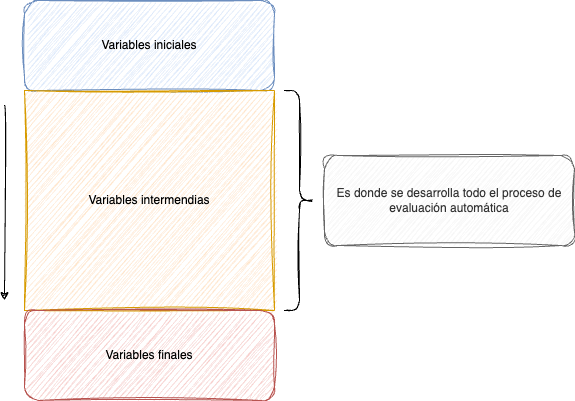
\includegraphics[width=0.7\linewidth]{Graphics/Tape}
	\caption{ Estructura básica de la cinta.}
	\label{fig:Tape}
\end{figure}

Para utilizar esta cinta en un problema como los problemas de enrutamiento de vehículos se debe definir, en primer lugar, las operaciones básicas (o reglas) que aparecerán en cada uno de los problemas. Como se presentan en el capítulo \ref{chapter: VRP}, sección \ref{3-Criterias}, se deben definir los criterios de vecindad que modificarán la solución. 

Estas operaciones se pueden usar en la cinta como ocurre con la Diferenciación automática. La modificación de cada operación se propaga solamente por las ramas que se afectan en cada variante del problema y no se afecta el sistema completo, sino solo ese subproblema, que se debe reevaluar. 

La relación entre las operaciones que se presentan en una función a la que se le aplicará la Diferenciación Automática y las operaciones que componen los criterios de vecindad permite que se utiliza la idea de esta cinta en ambos casos. Al aplicar el criterio de vecindad se obtiene una solución "derivada" de la solución inicial y las operaciones que la componen, al igual que en AD, quedan en la cinta para evaluar solo la parte modificada de la solución.

En este capítulo se presentó el procedimiento de diferenciación automática que utiliza además de un grafo de evaluación, una cinta automática para obtener la derivada de una función matemática.

En el siguiente capítulo se desarrolla esta idea de la diferenciación automática en la evaluación de soluciones vecinas de cualquier VRP.

% Chapter 3 Mezcla y código en Lisp

% Chapter 4 Resultados

% Conclusiones, recomendaciones y bibliografía




























